The conditioning process, consisting of cutting and polishing the fibers, is an individual task that generates a small dispersion in the response of each individual fiber, $\sigma_{con}$. This is an uncertainty that will be present in the tritium measurement of the monitor.

%The uncertainty of the conditioning process, $\sigma_{con}$, was experimentally measured. This uncertanty appeares because, as we saw before, each fiber have to be conditioned, consisting in cutting and polishing it, before using. This is an individual task that can present a small dispersion, affecting the response of each individual fiber. It is an important measurement because this uncertainty will be present in the TRITIUM detector.

To measure this dispersion, it has to be taken into account that the position of the connectors that lock the fiber in the experimental setup produce an additional uncertainty, $\sigma_{pos}$, in the measurement. Since both uncertainties are independent, the total uncertainty is given by:

\begin{equation}
\sigma_{t} = \sqrt{\sigma^2_{pos} + \sigma^2_{con} }
\label{eq:TotalUncertaintyFiberCharacterization}
\end{equation}

The uncertanty due to the fiber position has to be quantified to extract from the total uncertainty. Two different experiments were designed, the first with only the uncertainty in the fiber position ($\sigma_{t} = \sigma_{pos}$), and the second with both uncertainties. The conditioning uncertainty is given by:

\begin{equation}
\sigma_{con} = \sqrt{\sigma^2_{tot} - \sigma^2_{pos} }
\label{eq:ConditioningUncertaintyFiberCharacterization}
\end{equation}

The test designed to measure $\sigma_{pos}$ consisted of preparing one fiber of each type (uncladded, single clad and multiclad) by the conditioning process reported above. Each fiber was locked in the set up, and a measurement by feeding the LED with an intensity of $0.1~\milli\ampere$  was done. These measurements were repeated ten times with the same fiber. Ten different measurements for each fiber type was obtained. The standard deviation of the set of measurements is only due to the position uncertainty. The results are shown in Table \ref{tab:PositionStandardDeviation}.

\begin{equation}
\sigma^{rel}_{pos} = \frac{\sigma_{pos}}{\bar{x}}
\label{eq:RelativeStandardDesviation}
\end{equation}

\begin{table}[htbp]
%%\centering
\begin{center}
\begin{tabular}{|c|c|c|c|c|}
\hline
Fiber type & Mean ($\gamma$/ns) & $\sigma_{pos}$ ($\gamma$/ns) & $\sigma^{rel}_{pos}$ (\%)\\
\hline \hline \hline
Uncladded & $524.088 \pm 0.010$ & $17.65$ & $3.37$ \\ \hline
Single Clad & $1071.696 \pm 0.01$ & $9.07$ & $0.85$ \\ \hline
Multiclad & $949.930 \pm 0.026$ & $9.91$ & $1.04$ \\ \hline
\end{tabular}
\caption{Mean and standard deviation (due to fiber position in the setup) of photons per nanosecond that reach the PMT for $0.1~\milli\ampere$ LED intensity.}
\label{tab:PositionStandardDeviation}
\end{center}
\end{table}

As it can be seen, the clad reduces the position uncertainty, which means that it improves the uniformity of the fiber response. It was also found that the clad markedly improves the light collection efficiency of the fibers. The reason could be because photons are mainly collected in the core of the fiber and the interface of core and is better defined in the case of a single clad or multiclad fibers than for uncladded fibers. In the latter case, the interface is provided by the environment (air or water in the case of TRITIUM), and external conditions, as dirt, may produce noticeable interface fluctuations.

It is also see that a second clad slightly reduce the collection efficienciy. The reason could be that a second clad layer reduces the fiber core proportionally.

%We don't achieve any improvement with the second clad, which means that the photons are mainly collected in the core of the fiber.

%A possible reason of that is because, in the case of uncladded fibers, the state of the interface between the core and the environment (air or water in our case) is much more important than in the others, where the most important interface is the one created between the fiber core and the first clad, which could be the reason why the difference between the signals of single clad and multiclad fibers are too small.

Concerning the error of the measurement, the error of the Keithley device was three orders of magnitude smaller than the standard deviation, and it was not taken into account.

%In addition to the $\sigma_{pos}$ measurement, we have measured the number of photons collected by each type of fiber in the same situation, which is higher for single clad and even higher for multiclad. It means that the clad has an appreciable effect on the fiber collection efficiency and it could be a possible point to futur studies.

To determinate the whole uncertainty, ten different samples of each fiber type were prepared and each fiber was measured under the same conditions as the previous test. This measurement was done for four different LED emission intensities ($0.05$, $0.1$, $0.15$ and $0.2~\milli\ampere$) to reduce possibles mistakes. The results of uncladded fibers are plotted in Figure \ref{fig:10samplesNC}, where it can be seen that, although each fiber shows a very linear trend with the amount of collected photons, a dispersion in the fiber response is clearly seen. Similar results were obtained for single clad and multiclad fibers, displayed in figures \ref{subfig:10samplesSC} and \ref{subfig:10samplesMC} respectively.

\begin{figure}[h]
\centering
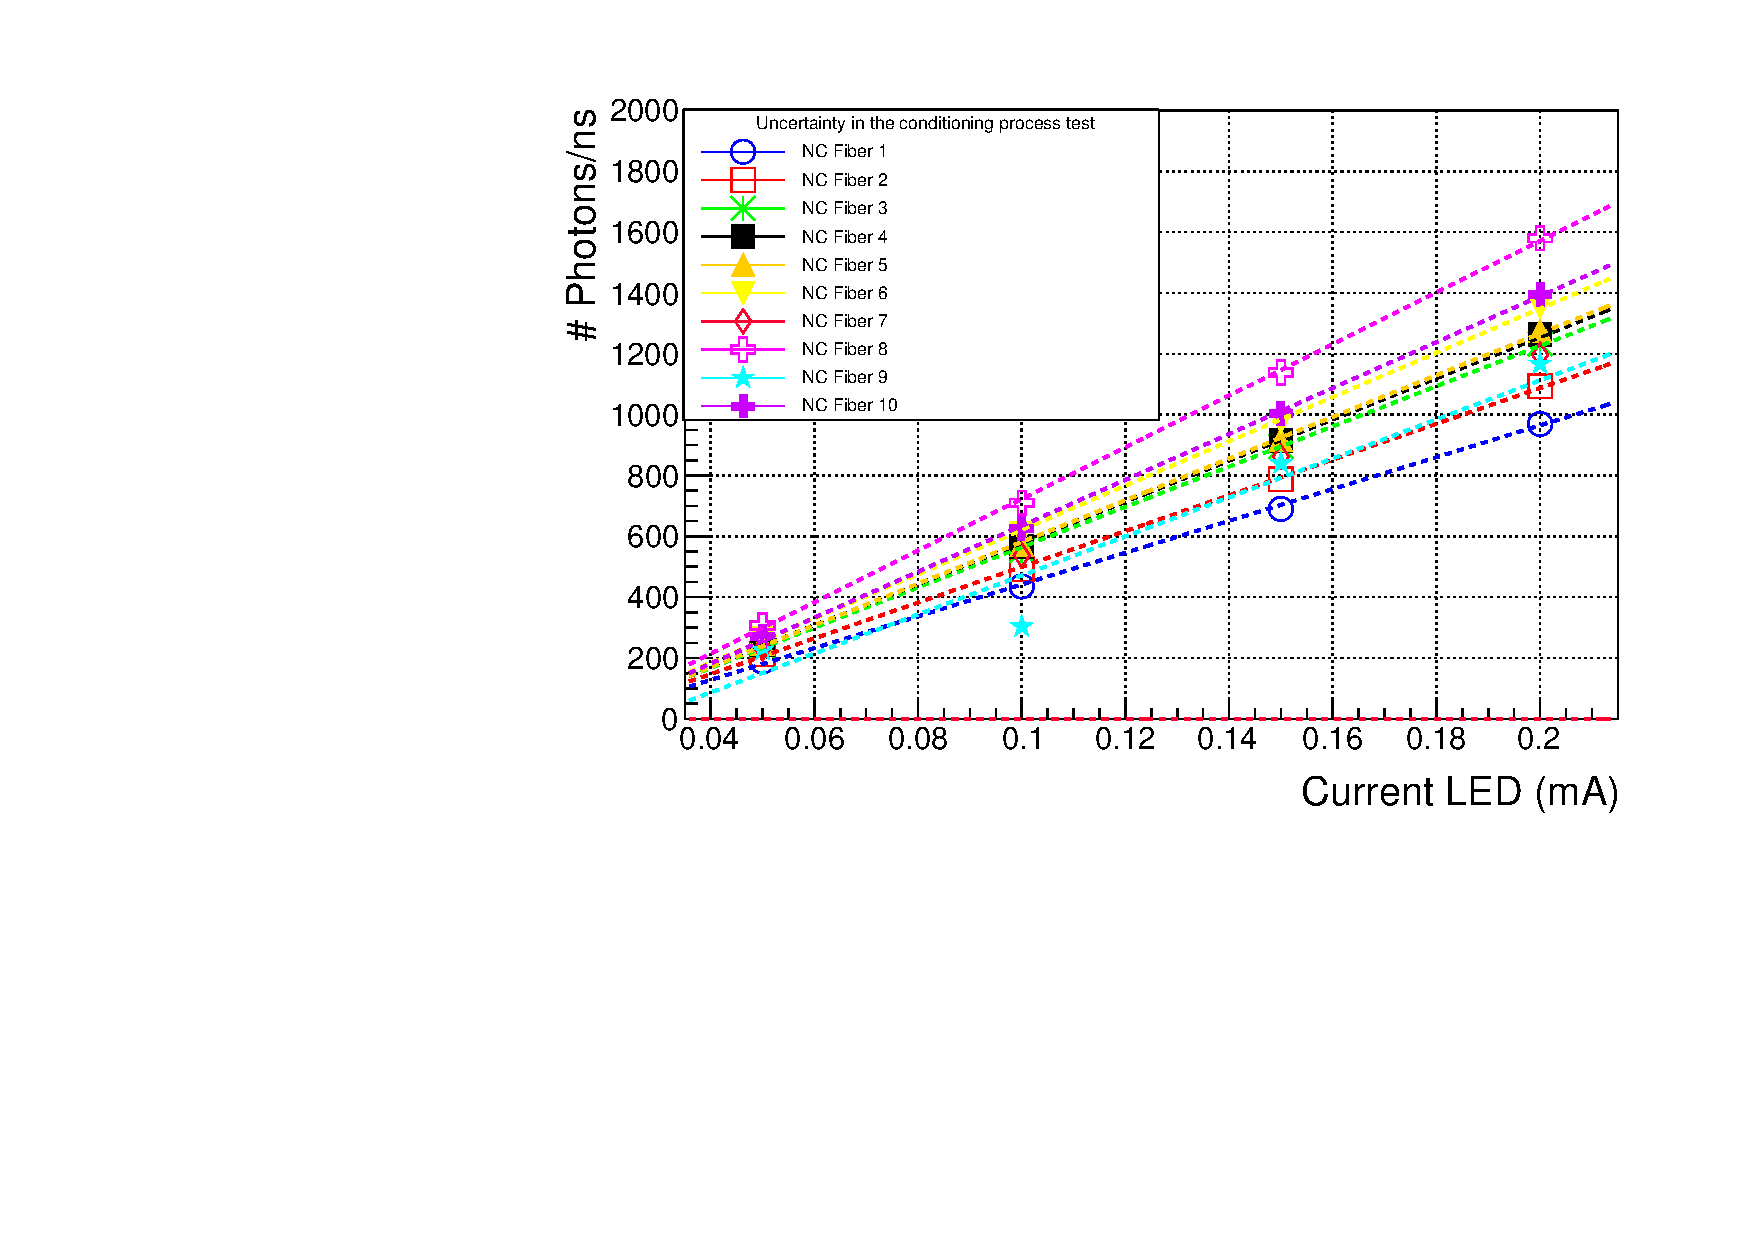
\includegraphics[scale=0.7]{4ResearchAndDevelopments/41Fibers/10_Different_samples_NoClad.pdf}
\caption{Number of photons/ns reaching the PMT for Uncladded fibers.\label{fig:10samplesNC}}
\end{figure}

\begin{figure}
\centering
    %\begin{subfigure}[b]{0.6\textwidth}
    %\centering
    %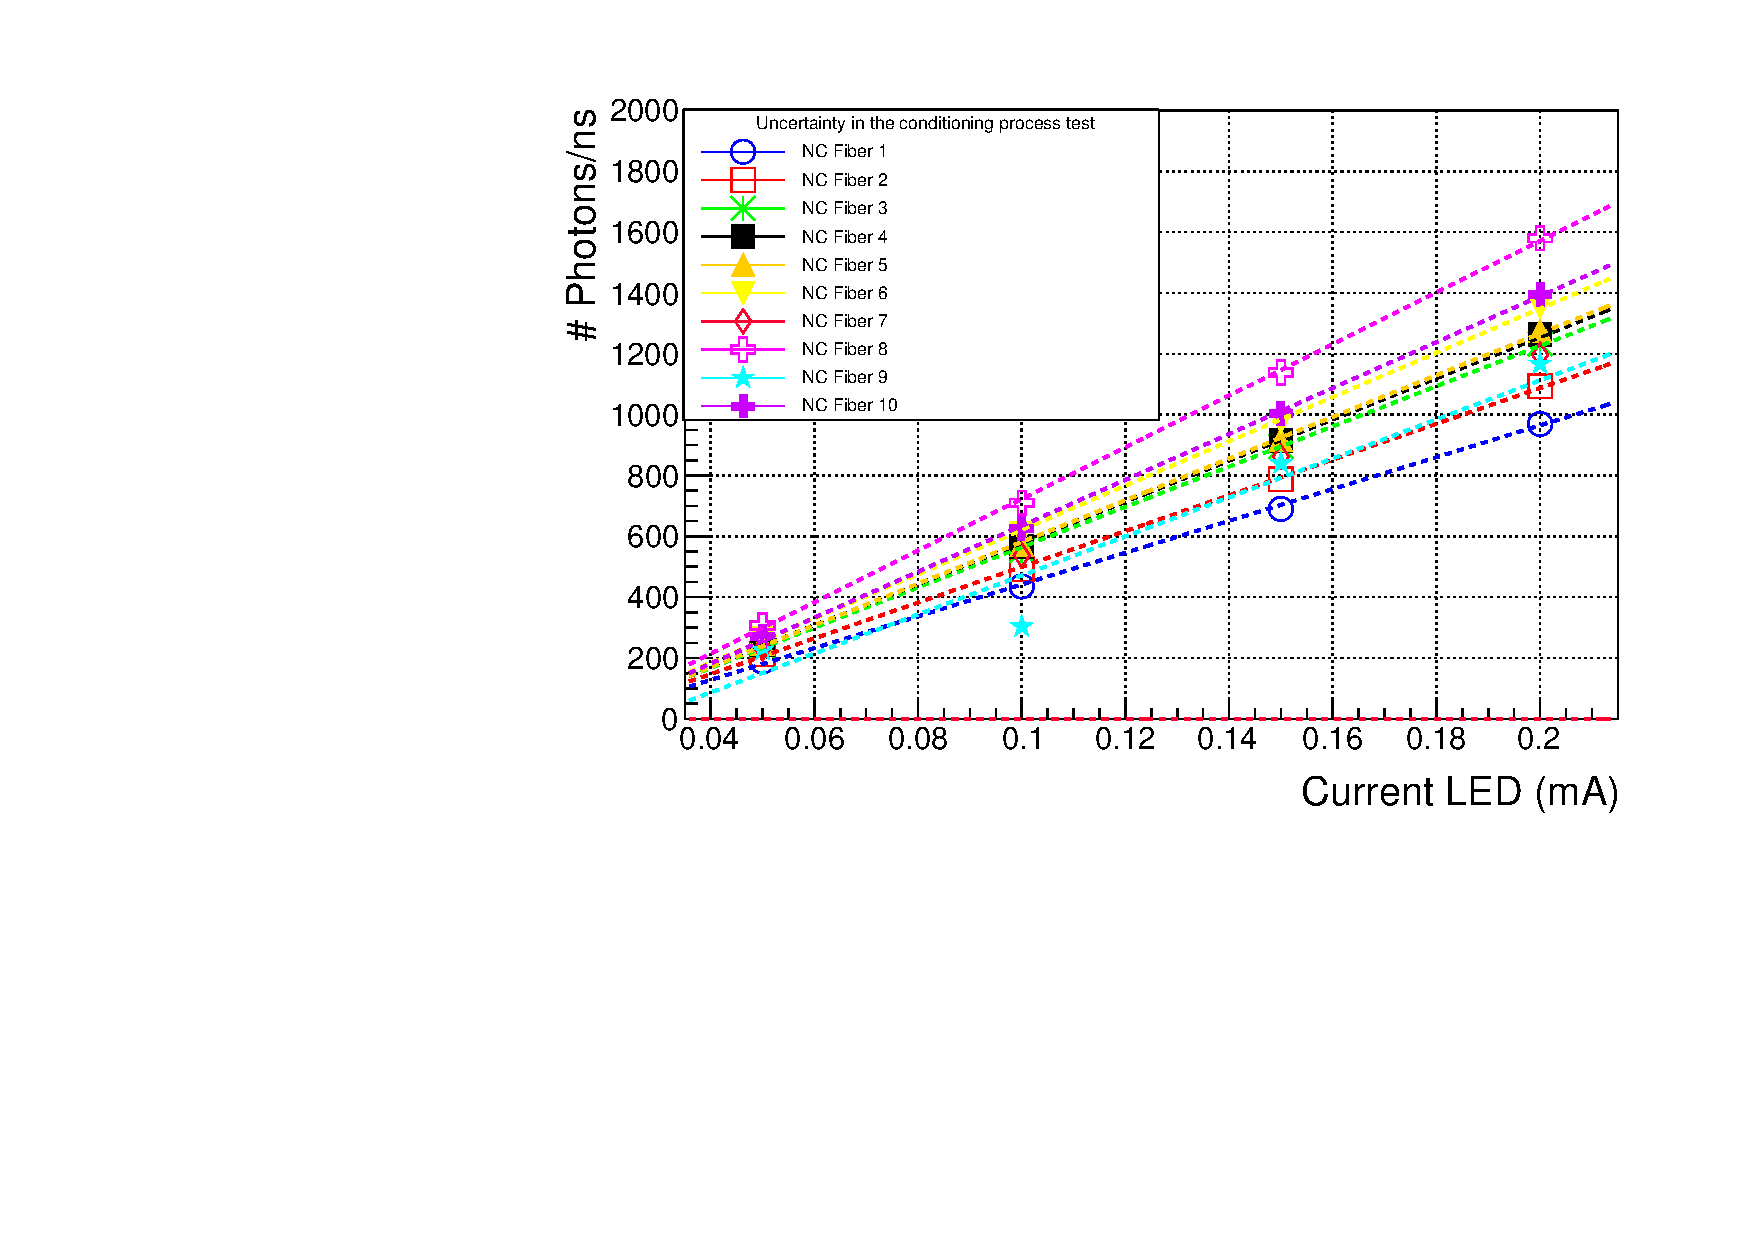
\includegraphics[width=\textwidth]{4ResearchAndDevelopments/41Fibers/10_Different_samples_NoClad.pdf}  
    %\caption{Number of photons/ns reaching the PMT for uncladded fibers.\label{subfig:10samplesNC}}
    %\end{subfigure}
    %\hfill
    \begin{subfigure}[b]{0.9\textwidth}
    \centering
    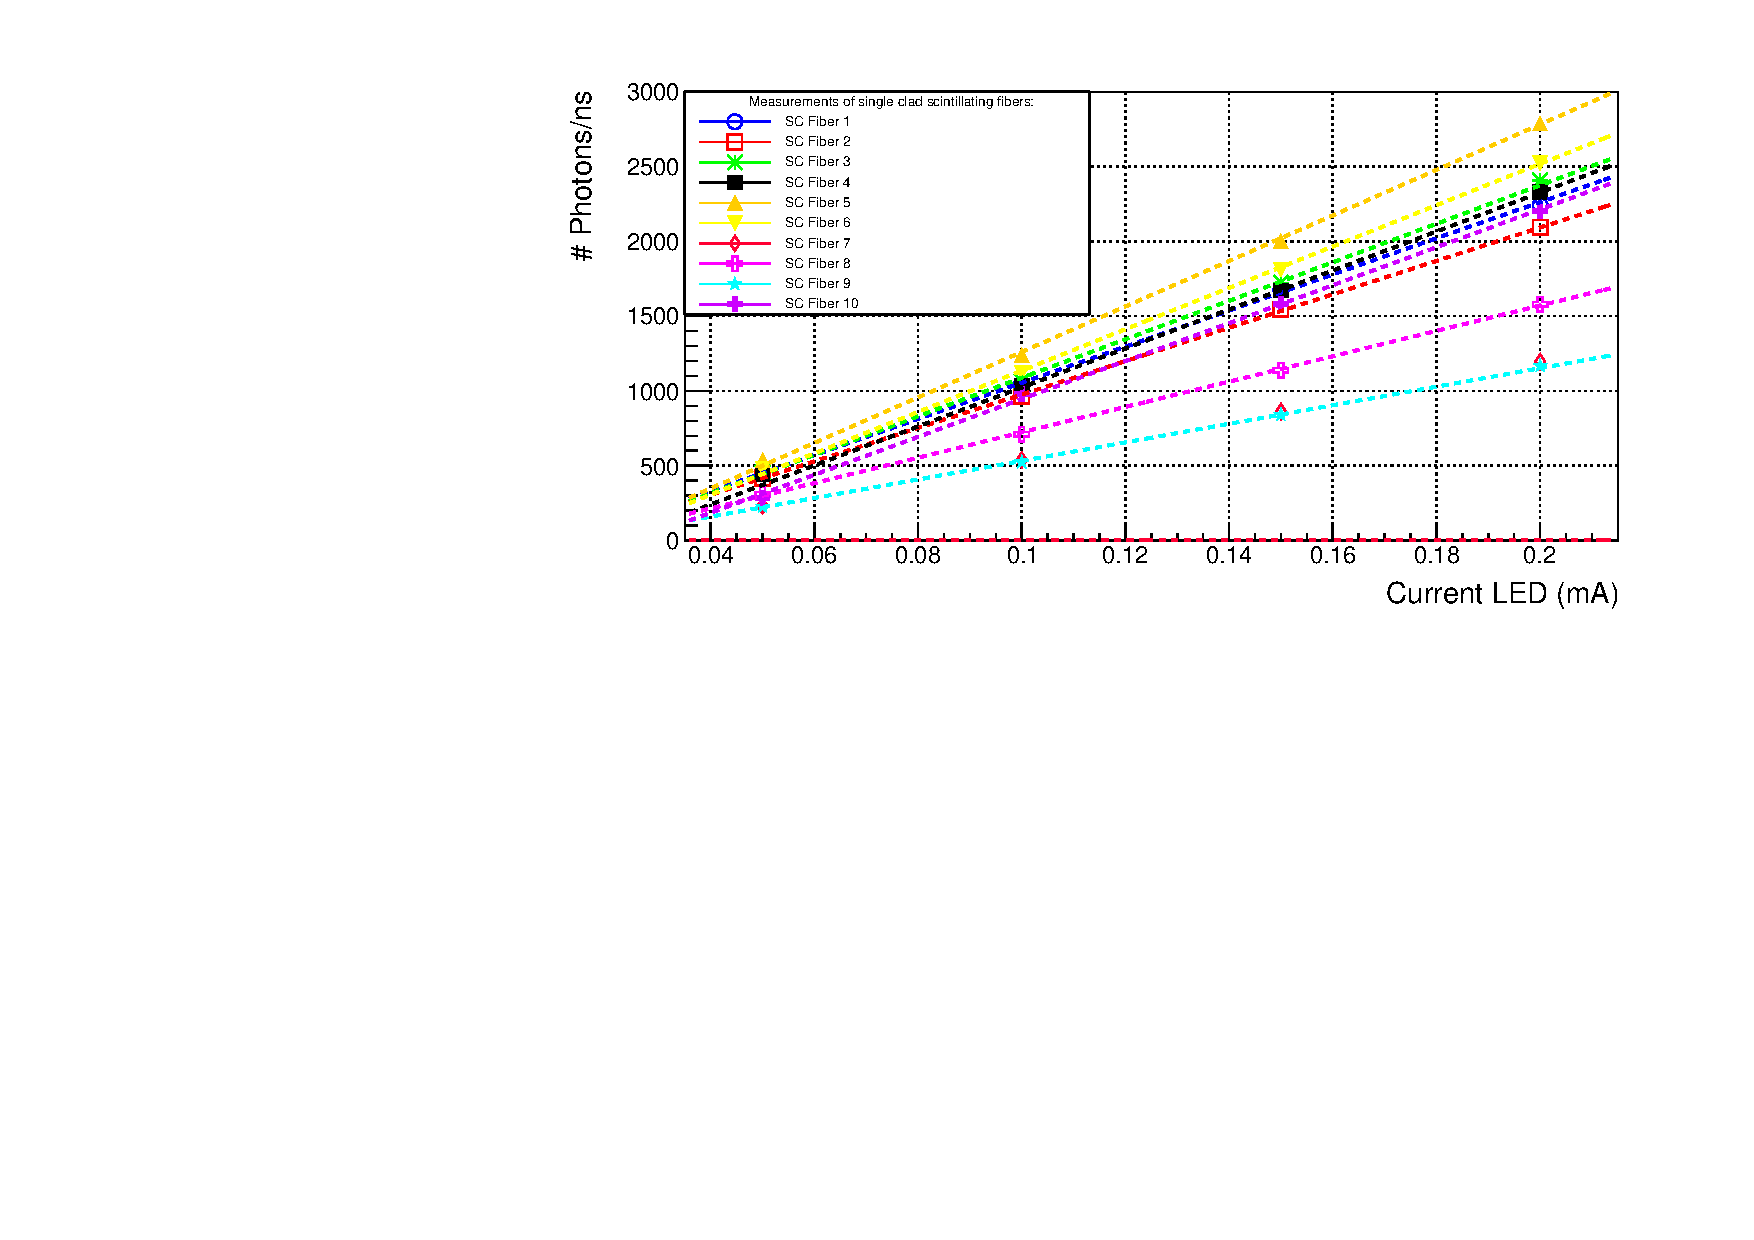
\includegraphics[width=\textwidth]{4ResearchAndDevelopments/41Fibers/10_Different_samples_SingleClad.pdf}  
    \caption{Number of photons/ns reaching the PMT for Single Clad fibers.\label{subfig:10samplesSC}}
    \end{subfigure}
    \hfill
    \begin{subfigure}[b]{0.9\textwidth}
    \centering
    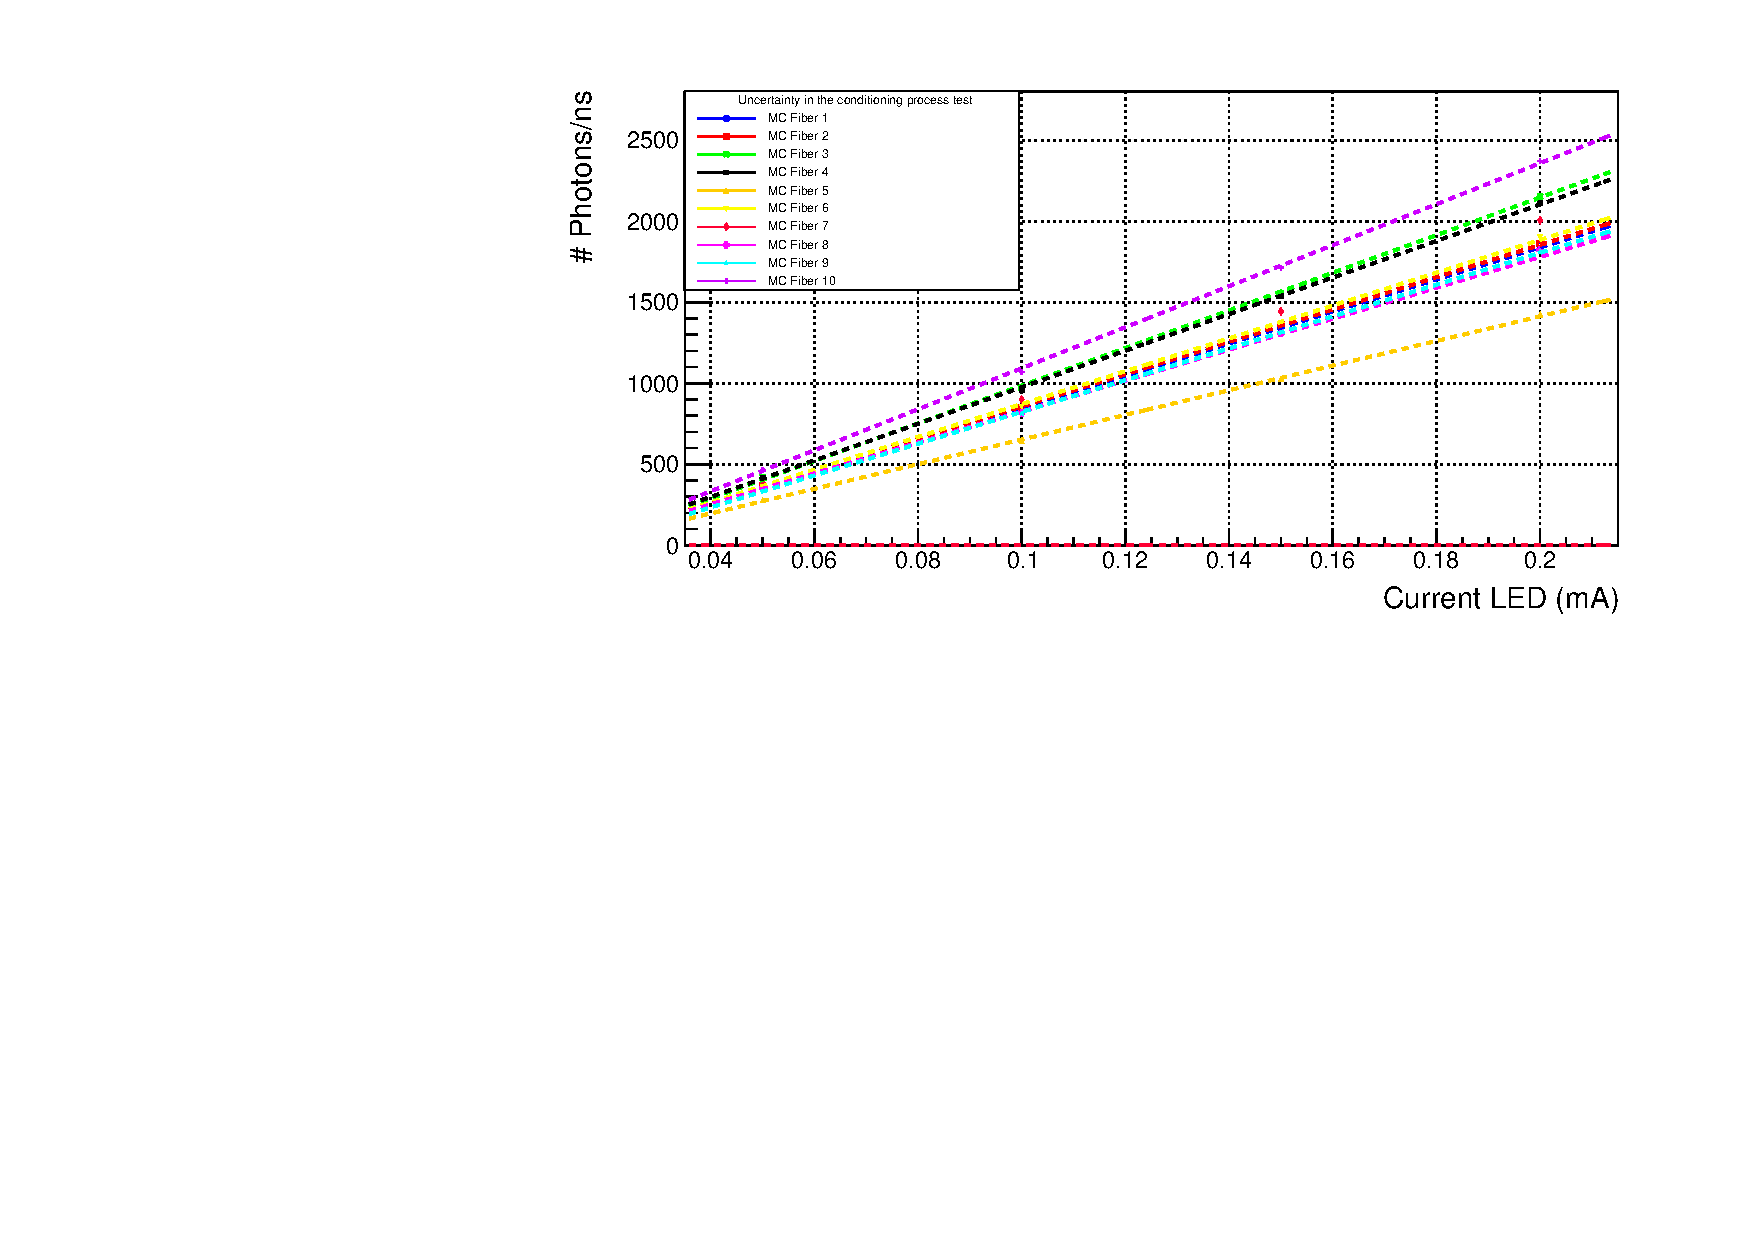
\includegraphics[width=\textwidth]{4ResearchAndDevelopments/41Fibers/10_Different_samples_MultiClad.pdf}  
    \caption{Number of photons/ns reaching the PMT for MultiClad fibers.\label{subfig:10samplesMC}}
    \end{subfigure}
 \caption{Number of photons/ns reaching the PMT for ten samples of each fibers type.}
 \label{fig:10samplesThreeTypes}
\end{figure}

The average number of collected photones versus LED intensity and the relative standard deviation for each type of fiber is given in Tables \ref{tab:10DifferentSamples} and \ref{tab:RelativeStandardDeviation3FiberTypes} respectively and represented in Figure \ref{fig:AveregeThreeFiberTypes}, where they can be compared. 

\begin{table}[h]
%%\centering
\begin{center}
\begin{tabular}{|c|c|c|c|c|}
\hline
Led Int. (mA) & Uncladded & Single Clad & MultiClad\\
\hline \hline \hline
$0.05$ & $243 \pm 10$ & $384 \pm 33$ & $377 \pm 15$ \\ \hline
$0.1$ & $541 \pm 34$ & $923 \pm 74$ & $871 \pm 35$ \\ \hline
$0.15$ & $903 \pm 37$ & $1485 \pm 120$ & $1397 \pm 55$ \\ \hline
$0.2$ & $1253 \pm 50$ & $2054 \pm 166$ & $1933 \pm 76$ \\ \hline
\end{tabular}
\caption{Number of the collected photons versus LED intensity for the different type of fibers.}
\label{tab:10DifferentSamples}
\end{center}
\end{table}

\begin{table}[h]
%%\centering
\begin{center}
\begin{tabular}{|c|c|c|c|c|}
\hline
Led Int. (mA) & Uncladded & Single Clad & MultiClad \\
\hline \hline \hline
$0.05$ & $4.03$ & $8.66$ & $3.97$ \\ \hline
$0.1$ & $6.20$ & $8.02$ & $3.97$ \\ \hline
$0.15$ & $4.08$ & $8.07$ & $3.95$ \\ \hline
$0.2$ & $4.03$ & $8.10$ & $3.93$ \\ \hline
Mean & $4.05$ & $8.21$ & $3.96$ \\ \hline
\end{tabular}
\caption{Relative standard deviation versus LED intensity for the different fiber types.}
\label{tab:RelativeStandardDeviation3FiberTypes}
\end{center}
\end{table}

\begin{figure}[h]
\centering
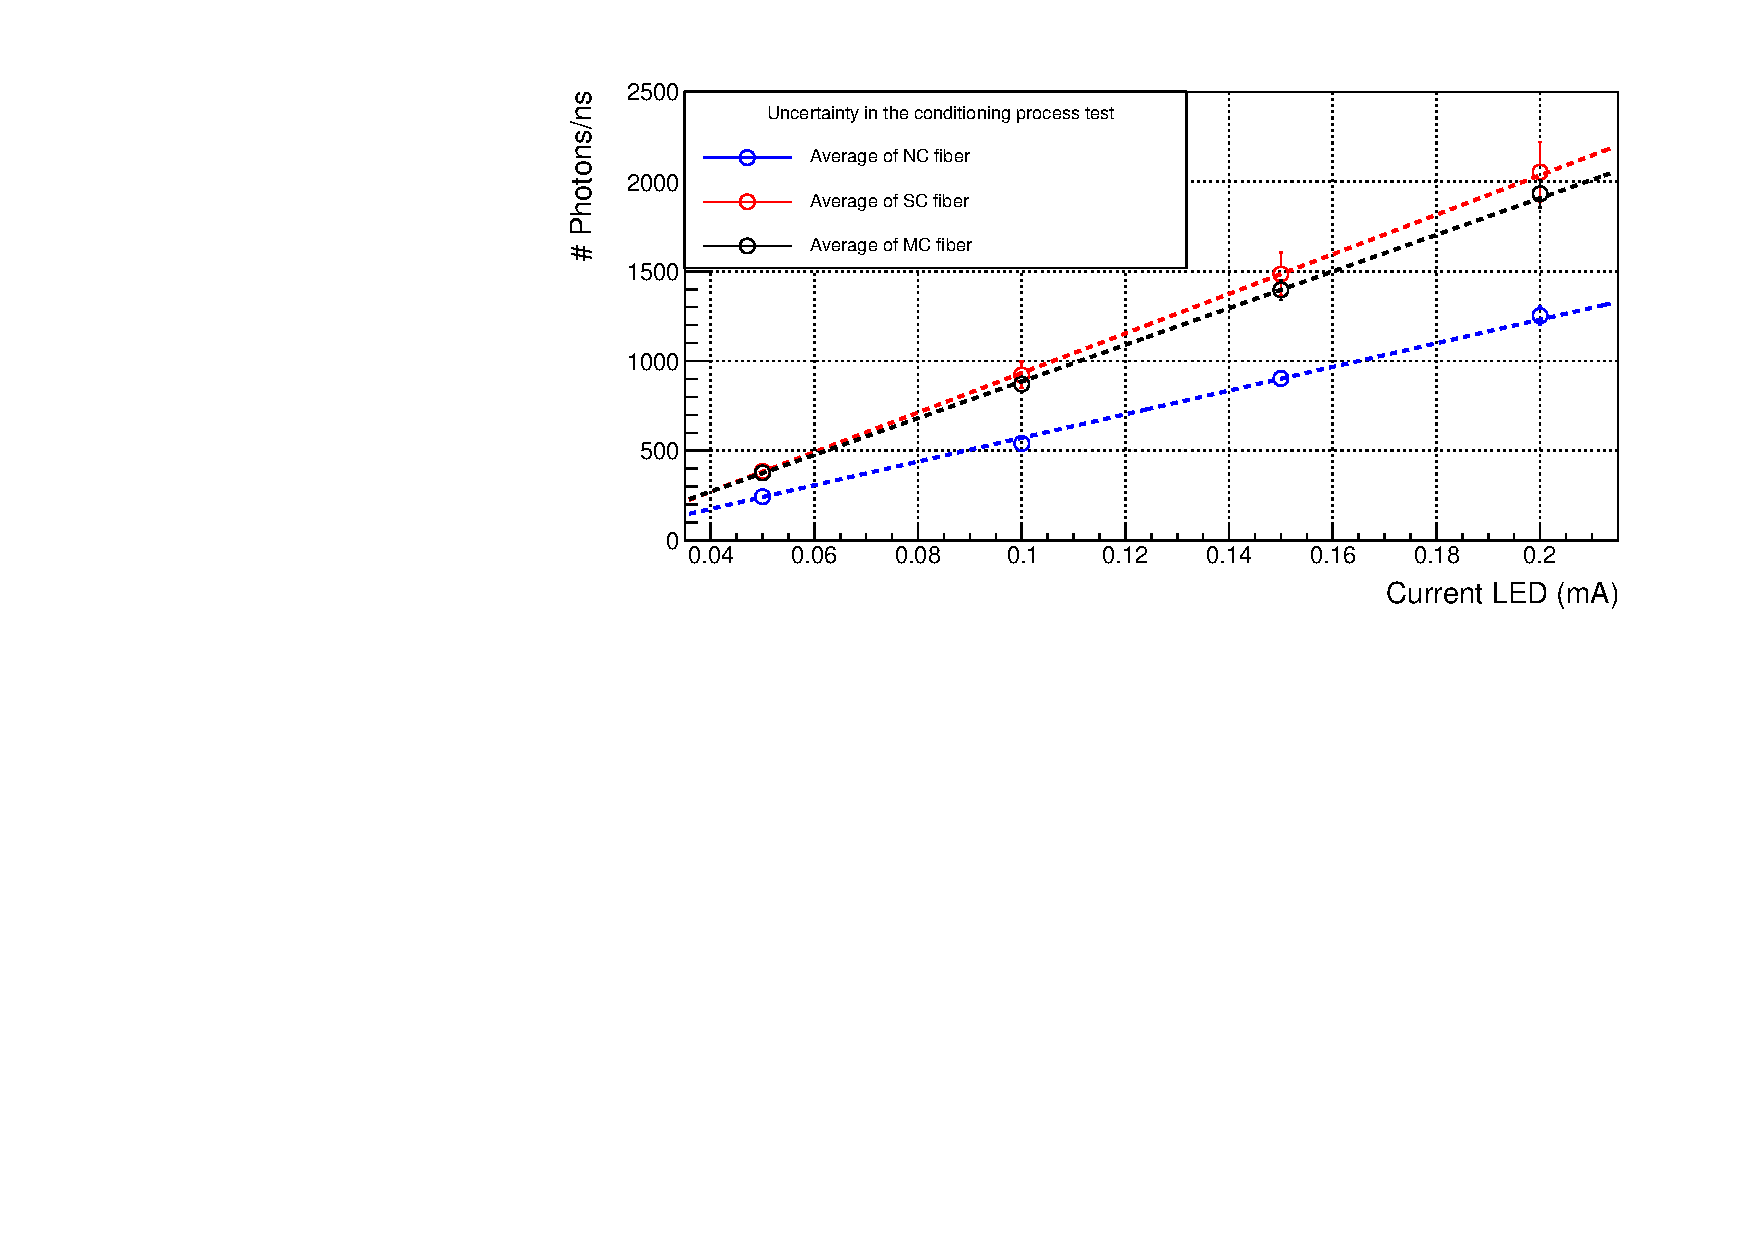
\includegraphics[scale=0.6]{4ResearchAndDevelopments/41Fibers/10_Different_Samples_Average_3_Fiber_Types.pdf}
\caption{Average of 10 samples for each fiber type (uncladded, single clad and multiclad fibers).\label{fig:AveregeThreeFiberTypes}}
\end{figure}

As it can be noticed in Figures \ref{fig:10samplesNC} and \ref{fig:10samplesThreeTypes} the fiber response is quite linear and that single clad and multiclad fibers have stronger signals that uncladded fibers, which means that the clad has a significant effect on the fiber collection efficiency. Also, it was found that single-clad fibers have higher collection efficiency than multiclad fibers. It can also remarked in Table \ref{tab:RelativeStandardDeviation3FiberTypes} that the relative standard deviation, $\sigma^{rel}_{pos}$, does not vary with the LED intensity.

%The relative standard deviation are also presented in these tables, where we it can be seen that the dispersion of each fiber type for different LED intensities is practically negligible, which again verifies the correct behavior of the system. 

%There is only one point (uncladded fiber with $0.1~\milli\ampere $) that is higher than we expect. We can see in Table \ref{tab:10DifferentSamplesNoClad} that the reason for this is that its standard deviation is too high (as high as the measurement for uncladded fibers with $0.15~\milli\ampere$). The reason was found in the sample 9, whose measurement was very different from the average, incresing the standard deviation, probably due to a problem in the measurement process. We discard this sample because this result is not representative.

An average of the uncertainty due to the fiber position and the conditioning process are given in Table \ref{tab:RelativeStandardDeviations}.

\begin{table}[htbp]
%%\centering
\begin{center}
\begin{tabular}{|c|c|c|c|}
\hline
Fiber type & $\sigma_t$ (\%) & $\sigma_{pos}$ (\%) & $\sigma_{con}$ (\%)\\\hline \hline \hline
Uncladded & $4.05$ & $3.37$ & $2.25$ \\ \hline
Single Clad & $8.21$ & $2.17$ & $7.92$ \\ \hline
Multiclad & $3.96$ & $1.04$ & $3.82$ \\ \hline
\end{tabular}
\caption{Relative standard deviations ($\sigma_t$, $\sigma_{pos}$ and $\sigma_{con}$) measured in this test.}
\label{tab:RelativeStandardDeviations}
\end{center}
\end{table}

As it can be seen, the smallest uncertainty in the conditioning process was found in the uncladded fibers, which means that the damage from this process occurs mainly in the fiber clad, as can be checked in Figure \ref{fig:ResultofPolishingProcess}. It was checked under the microscope that this damage only occurs at the end of the fiber. Also, the largest relative standard deviation in this process is measured for single clad fibers, which means that the second clad increases the resistance of the fiber to the conditioning process.

In summary, this study has shown that the use of fiber clad improves the photon collection efficiency. The relative statistical deviation due to the fiber conditioning process was quantified for the different fiber types. It was found that the damage of the conditioning process is produced mainly in the fiber clad. Thus, if a method to build a clad for fibers is developed, it should be applied after the fiber conditioning process.

Finally, the measurement of the photon collection efficiency of each type of fiber is shown. The collection efficiency is the percentage of photons collected along the fibers. It is usually given by $1~\meter$ fiber length, $CE_ {100}$.

To measure the collection efficiency, $CE_{100}$, ten different samples $10~\cm$ length was prepared for each fiber type. The results are given in Table \ref{tab:10DifferentSamplesAlltypes}.

\begin{table}[htbp]
%%\centering
\begin{center}
\begin{tabular}{|c|c|c|c|c|}
\hline
Led Int. (mA) & Uncladded ($\gamma$/ns) & Single clad ($\gamma$/ns) & MultiClad ($\gamma$/ns) \\
\hline \hline \hline
$0.05$ & $318 \pm 61$ & $550 \pm 71$ & $480 \pm 84$ \\ \hline
$0.1$ & $736 \pm 143$ & $1270 \pm 164$ & $1111 \pm 193$ \\ \hline
$0.15$ & $1184 \pm 232$ & $1984 \pm 231$ & $1777\pm 307$ \\ \hline
$0.2$ & $1645 \pm 324$ & $2507 \pm 208$ & $2338 \pm 350$ \\ \hline
\end{tabular}
\caption{Number of the collected photons versus LED intesntity for 10 different fibers of $10~\cm$ length.}
\label{tab:10DifferentSamplesAlltypes}
\end{center}
\end{table}

%The collection efficiency can be calculated by comparing these tests with those performed for a fiber length of $20~\cm$, whose values has been previously shown in Tables \ref{tab:10DifferentSamplesNoClad}, \ref{tab:10DifferentSamplesSingleClad} and \ref{tab:10DifferentSamplesMultiClad} since both was made under the same conditions. The results is shown in Table \ref{tab:CollectionEfficiencyOfFibers}:


%Due to the reason that both tests were run in the same setup under exactly the same conditions, the difference between both situations is the photons per nanosecond that have not been collected in this extra $10~\cm$ of fiber. Therefore, using the equation \ref{}, the collection efficiency in $10~\cm$ of fiber can be calculated for each sort of fiber, whose result is shown in the last column.

The collection efficiency in $10~\cm$ fiber length, $CE_{10}$, was calculated by comparing these tests with those performed for a fiber length of $20~\cm$ and the collection efficiency, $CE_{100}$, was calculated from $CE_{10}$ by assuming a linear deppendance on length.

\begin{table}[htbp]
%%\centering
\begin{center}
\begin{tabular}{|c|c|c|}
\hline
Fiber type & $CE_{10}$ (\%) & $CE_{100}$ (\%) \\\hline \hline \hline
UnCladded & $76 \pm 8$ & $7.6 \pm 0.8$ \\ \hline
Single Clad & $78 \pm 6$ & $7.8 \pm 0.6$ \\ \hline
Multiclad & $83 \pm 7$ & $8.3 \pm 0.7$ \\ \hline
\end{tabular}
\caption{Collection efficiencies $CE_{10}$ and $CE_{100}$.}
\label{tab:CollectionEfficiencyOfFibers}
\end{center}
\end{table}

%As the difference between the fiber length in both studies is only $10~\cm$, the collection efficiency calculated from these measurements, $CE_{10}$, is only at that distance. Assuming a linear dependence of this parameter with the distance, the value of $CE_{100}$ can be extrapolated.

The collection efficiency, $CE_{100}$, given by the manufacturer Saint-Gobain is between 7\% and 3.44\% \cite{DataSheetBCF12Fiber}. As collimated photons were used in this study, the fact that our results are in the best side is justified. As it can be seen in Table \ref{tab:CollectionEfficiencyOfFibers}, our measured values are very close to those provided by the manufacturer. %The difference between this value for the three types of fiber studied is not as large as it was expected. A possible reason is that the difference in fiber length is only $10~\cm$ and it may not be enough to see this effect. It could be interesting to repeat these tests with a larger difference in fiber length.